% !TEX root = ../main.tex

\chapter{Results Evaluation}

This chapter discusses results provided by the developed system and how they answer the questions posed at the beginning of this project. The full set of data looked at is stored in the appendix \ref{appendix:dataAppendix}.

\section{Examined Entity}

The entity that will examined is a company called Gamestop. Gamestop is an American video game, consumer electronics, and gaming merchandise retailer. It is the largest video game retailer worldwide.

\begin{figure}[h!]
    \centering
    
\includegraphics[width=15cm,height=4cm,keepaspectratio]{resultsEvaluation/gamestop.png}
    \caption{Gamestop Logo}
    \label{fig:gamestop}
\end{figure}

The main reason for choosing this company is due to the fact that it has historically been a relatively stable company. However, an interesting sentiment fuelled phenomenon happened recently. In January of 2021, the company stock prices increased by 1,500\% over the course of two weeks due to a short squeeze mainly attributed to the members of a subreddit, r/wallstreetbets. Reddit is a social news aggregation, web content rating, and discussion website, and a subreddit is a channel within this website which specialises in a given topic. In this case a subreddit dedicated to stocks with high market risk. This seems to indicate that the stock prices of Gamestop were heavily driven by sentiment. Making this an exceptional case-study for this project.

\section{Descriptive Statistics}

The first step towards understanding the data-set is to understand each of the columns by themselves. This first step that may be used is to create an outline of the data-set using descriptive statistics, alongside a graph. This lays out the data in such a way were time is not an element and simply the general trends of the data can be understood. A part of this analysis is to attempt to understand whether these general trends have remained consistent. Therefore, various time spans are examined alongside the data-set as a whole. The time-spans examined here are the entire data-set and the past year worth of data.

\subsection{Price Columns}

The columns which give the most amount of information are:
\begin{itemize}
    \item Closing Prices
    \item 1 Day Returns
\end{itemize}

\begin{figure}[h!]
    \centering
    \subfigure[]{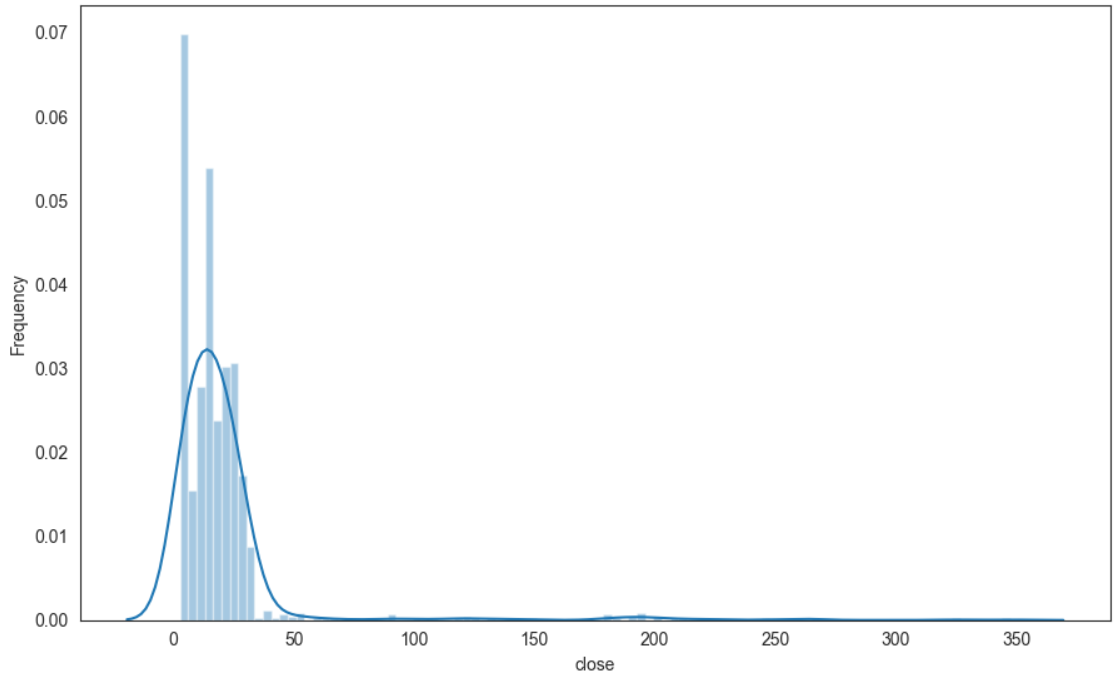
\includegraphics[width=0.49\textwidth,height=4cm]{resultsEvaluation/closeDescMax.png}}
    \subfigure[]{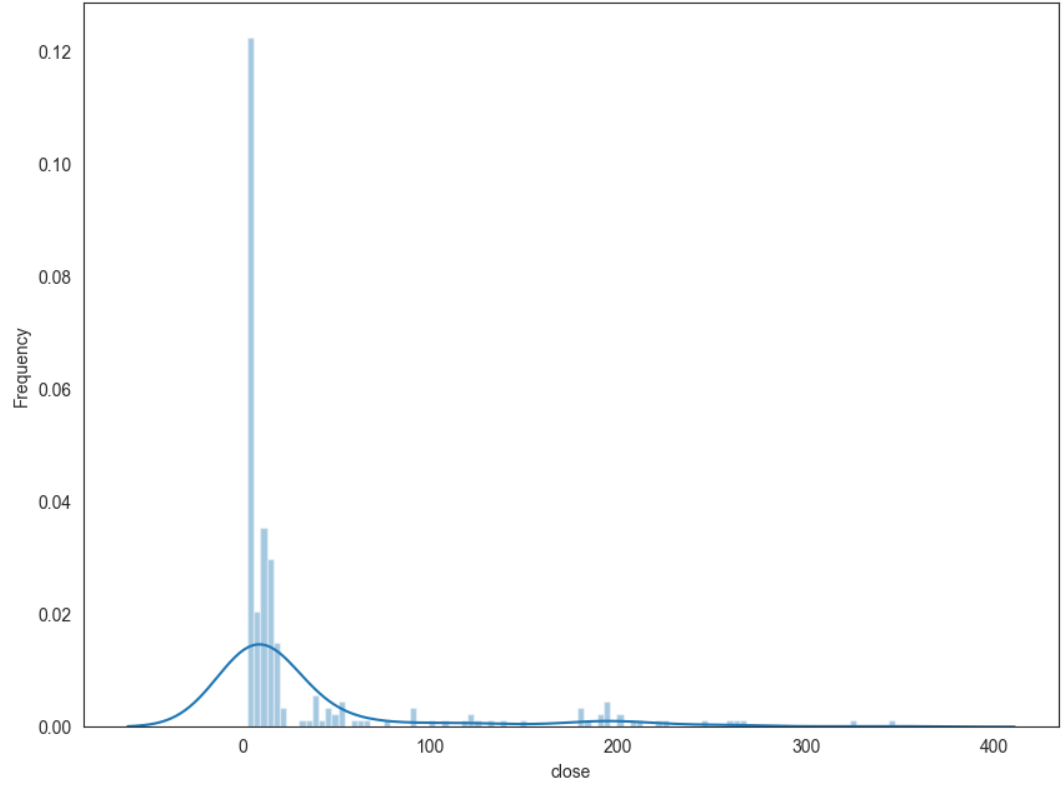
\includegraphics[width=0.49\textwidth,height=4cm]{resultsEvaluation/closeDesc1.png}}
    \caption{Closing Prices (a) entire data-set (b) last year of data}
    \label{fig:closeDesc}
\end{figure}

The first column examined is the closing price column. The initial observations from the overall dataset are:
\begin{itemize}
    \item There is a heavy left skew, confirmed with a skewness value of 6.0809, evidenced with a mean of 20.2554 when the standard deviation is 30.5661 and the minimum value is 2.8 while the maximum value is 347.51
    \item There are long tails, confirmed with a kurtosis value of 43.0012 and a range of 344.71 when the standard deviation is 30.5661
    \item There is a large concentration of points in the one area, making it unimodal, evidenced by a standard error of 0.8618
\end{itemize}
The data-set which includes only the last year of data-points compares in the following ways. The overall value of the closing prices has increased to having a mean of 35.3204 from 20.2554. However the most common values do lie in the same are as the mode went from 4.14 to 4.44, indicating that in general the price stayed the same. The median went from 15.22 to 10.22, actually decreasing a little bit, indicating that the much higher highs were balanced by much lower lows. The heavy left skew is maintained, it is however diminished with a new skewness value of 2.5837. This can partially be explained by the maximum and minimum values being the same, and the large amount of curve flattening seen by the standard error increasing to 4.0341 from 0.8618, the standard variance increasing to 4117.2946 from 935.0304. Similarly, the tails are still long given the kurtosis value of 6.1112, and the maintenance of the same range. However, the tails have more values within. All of this combined indicates that in the last year the stock's closing price has been far more volatile that usual, with the highest highs and lowest lows in the range examined. It seem that it has generally increased in value given the new mean. However, it is still hovering around the same price given the mode and median.

\begin{figure}[h!]
    \centering
    \subfigure[]{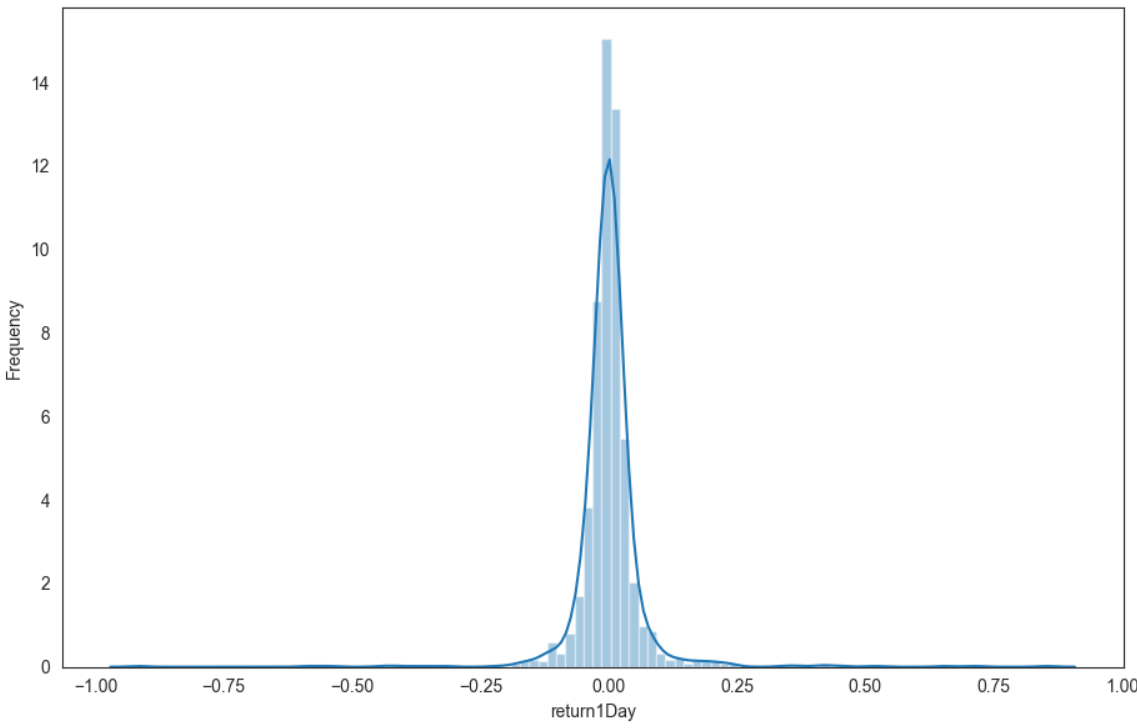
\includegraphics[width=0.49\textwidth,height=4cm]{resultsEvaluation/1returnDescMax.png}}
    \subfigure[]{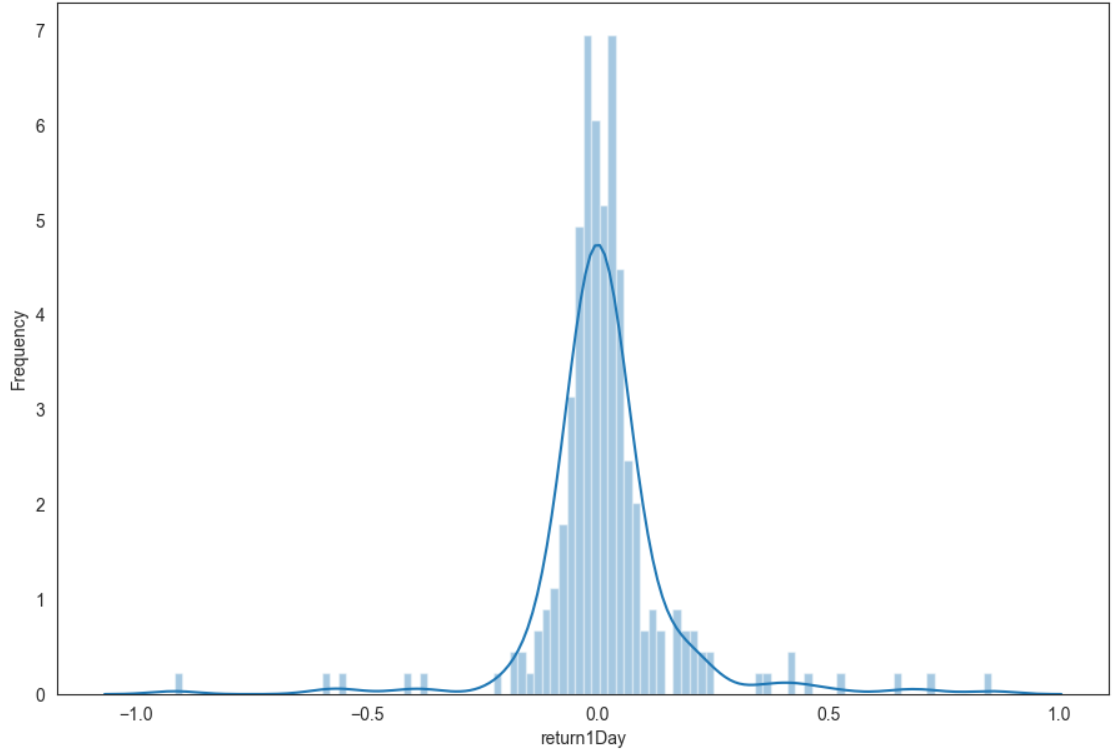
\includegraphics[width=0.49\textwidth,height=4cm]{resultsEvaluation/1returnDesc1.png}}
    \caption{1 Day Returns (a) entire data-set (b) last year of data}
    \label{fig:1returnDesc}
\end{figure}

The 1 day returns column is also examined. The initial observations are:
\begin{itemize}
    \item There is little to no skew, confirmed with a skewness value of 0.7638
    \item There are long tails, given the kurtosis value of 51.5650 and evidenced with the range of 1.7700 with a standard deviation of 0.0755
    \item There is a large concentration of points in the one area, making it unimodal, and evidenced with a standard error of 0.0021
\end{itemize}
The examination of the full data-set confirms the points made for closing prices. The mean, mode and median are all increased to 0.0162, 0.0053 and 0.0223 from 0.0014, 0.0 and 0.0. Indicating higher returns than over the entire data-set, however, this is marginal. Similarly as with closing process the skewness remains quite similar, to 0.7638 from 0.3239, where the decrease may be attributed to the increased flatness of the curve, seen by the standard error increase to 0.0096 from 0.0021. As well as this the tails are kept long, seen in the kurtosis value of 12.8680, and the same range being maintained. This information confirms the points laid out for closing prices.

\subsection{Sentiment Columns}

\begin{figure}[h!]
    \centering
    \subfigure[]{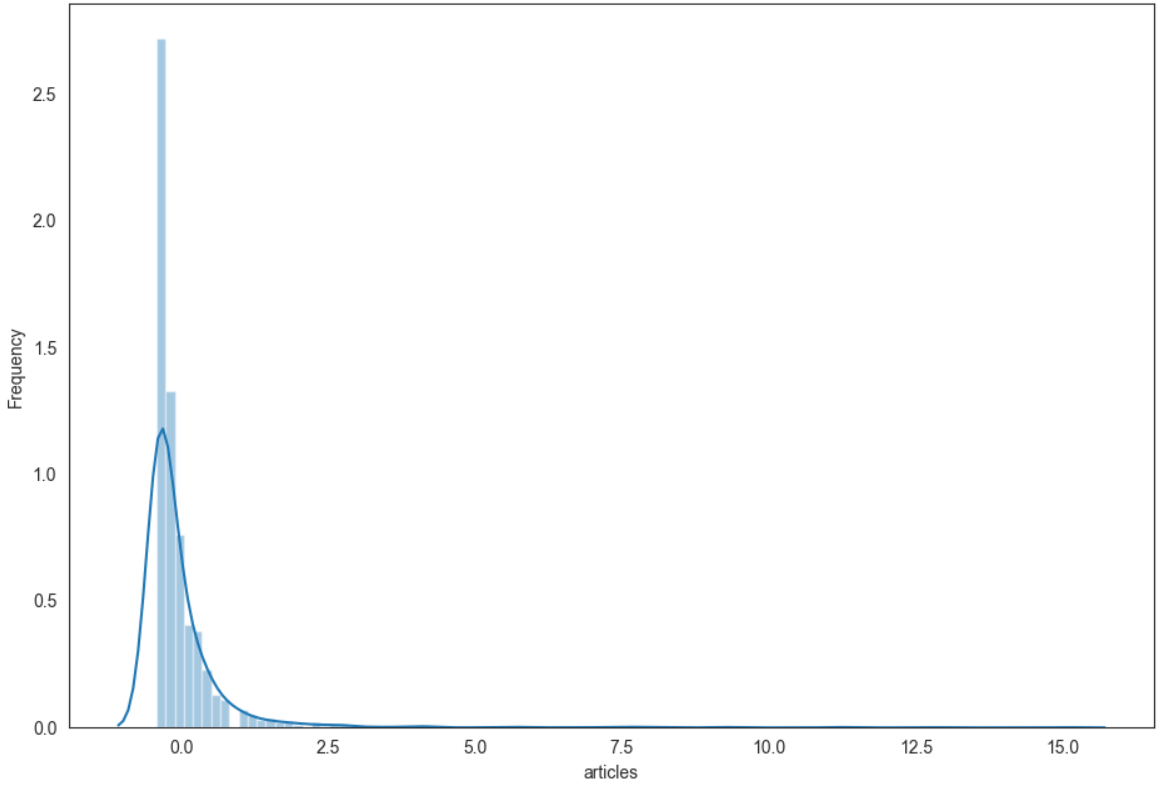
\includegraphics[width=0.49\textwidth,height=4cm]{resultsEvaluation/articleDescMax.png}}
    \subfigure[]{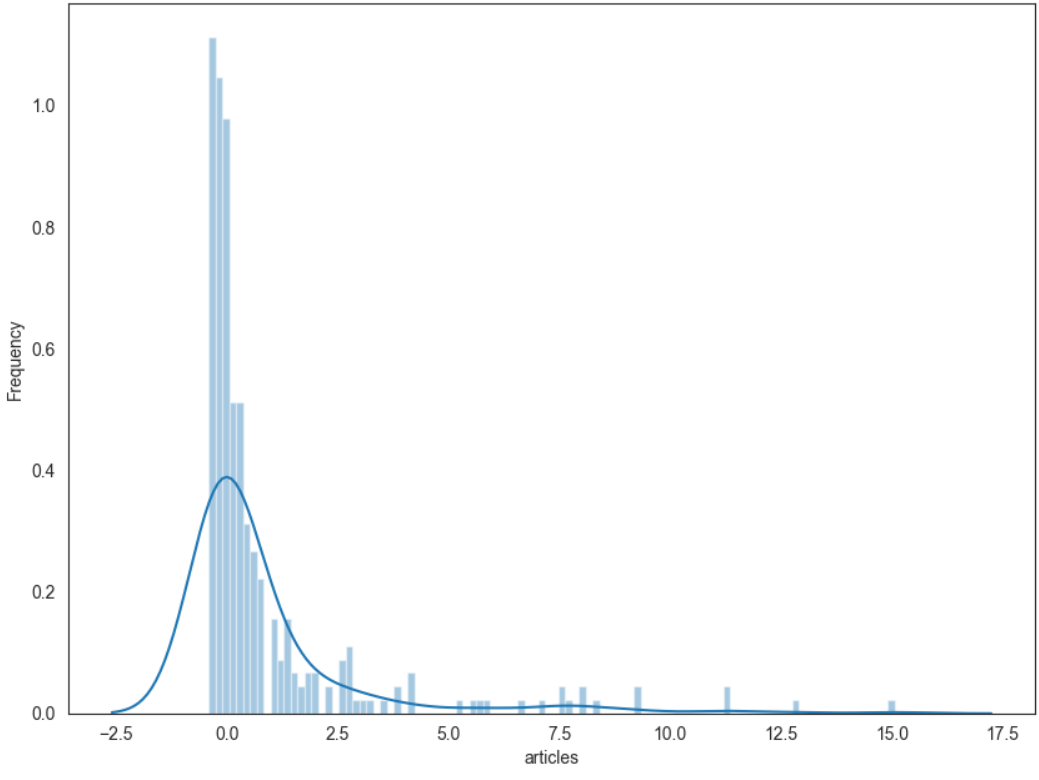
\includegraphics[width=0.49\textwidth,height=4cm]{resultsEvaluation/articleDesc1.png}}
    \caption{Article Volume (a) entire data-set (b) last year of data}
    \label{fig:articleDesc}
\end{figure}

The first column examined from the sentiment columns is the article volume column. The initial observations from the full data-set are:
\begin{itemize}
    \item There is a heavy left skew, confirmed by the skewness value of 7.3609
    \item There are long tails, given by the kurtosis value of 73.7692 and the range of 15.4788 and standard deviation of 1.0
    \item There is a large concentration of points in one area, making it unimodal, and evidenced with a standard error of 0.0220
\end{itemize}
The data-set which only takes into account one year is then considered. The mean and median are raised to 0.8623 and 0.1096 from 0.0 and -0.2422, meanwhile the mode is maintained constant at -0.4181. This indicates that there are more higher values, however, most of them are still concentrated in the same area. The other difference to point out is that flattening of the curve, indicated in the change of standard error to 0.1325 from 0.0220. The tailness maintained but slightly decreased due to the flattening of the curve, seen in the change of kurtosis to 12.2162 from 73.7692. The changes indicate that in the last year there was was more variation in the number of article towards the high-end, however, the majority of points remain the same. This aligns with what is seen in the prices and returns, which indicates some correlation between the two aspects.

\begin{figure}[h!]
    \centering
    \subfigure[]{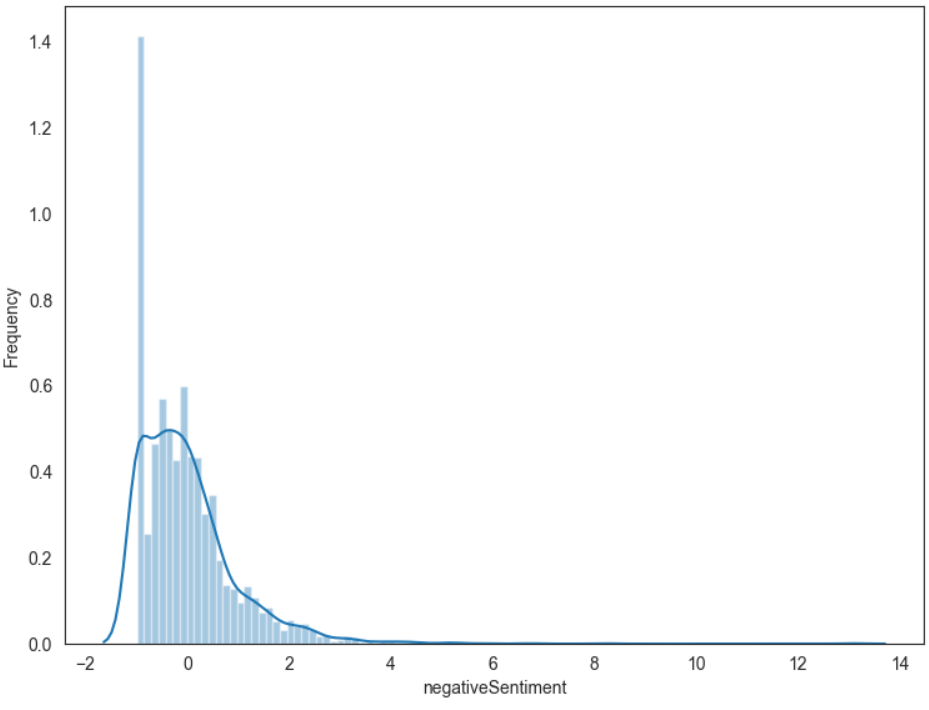
\includegraphics[width=0.49\textwidth,height=4cm]{resultsEvaluation/negativeDescMax.png}}
    \subfigure[]{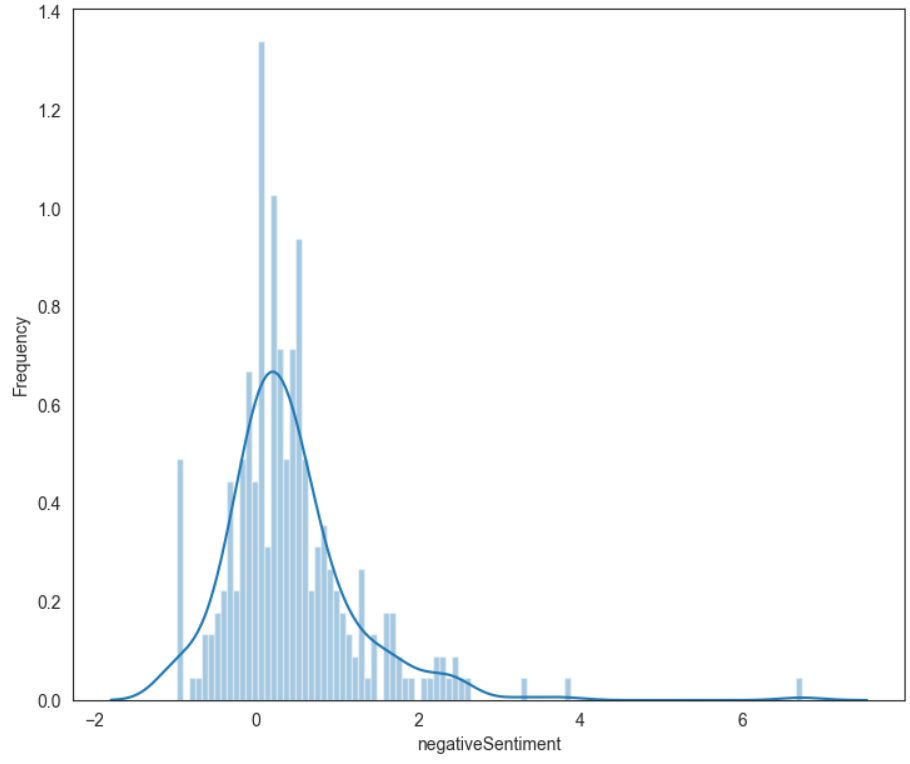
\includegraphics[width=0.49\textwidth,height=4cm]{resultsEvaluation/negativeDesc1.png}}
    \caption{Negative Sentiment (a) entire data-set (b) last year of data}
    \label{fig:negativeDesc}
\end{figure}

The next column examined is the negative sentiment column. The positive and negative sentiment column behave very similarly. So only one of these is examined. The initial observations are:
\begin{itemize}
    \item There is a left skew, confirmed by the skewness value of 2.7791
    \item There are long tails, given by the kurtosis value of 19.5138 and the range of 14.05 and standard deviation of 0.9998
    \item The data is concentrated around one area, making it unimodal, and evidenced with a standard error of 0.0220
\end{itemize}
The 1 year data-set compare in the following ways. The mean, median and mode all increase to 0.4129, 0.27 and 0.08 from 0.0001, -0.17 and -0.99. This indicates a general increase in negative sentiment in the last year. The curve flattened a small amount in the year given the change of standard error to 0.0489 from 0.0220. Unlike the rest of the examined columns however, the range of data is significantly decreased to 7.72 from 14.05, where the minimum remained the same at -0.99, and the maximum decreased from 13.06 to 6.73. These items seem to indicate that the general sentiment was more negative more regularly, however, it never reached the extremes that it previously had. It is interesting to note that a similar pattern occur when positive sentiment is examined. This seems to indicate that when there is more volatility in the market, and a larger amount of articles, the sentiment is generally higher, negative and positive.

It is important to note that preceding information indicates that the examination is conditional on the time-span examined for this data-set. This is due to the fact that the descriptive statistics change significantly depending on the time-span chosen.

\section{Auto Correlation}

This step in understanding the data-set continues the understanding of columns by themselves. However, it examines the relationship of the columns with themselves. It does this by finding the correlation of a column entry with a previous entry given a lag time. For example if the lag is 5, it will find the correlation with 5 entries prior, i.e. 5 days before. This is important to understand whether previous days have any correlation, and potentially an effect on the current day. For the purposes of this examination, the lag looked at is 5 for all items. In this section a p-value of 0.1 or smaller is going to be considered of statistical significance. The p-value indicates the probability of a non-correlated system producing data-sets that have a correlation at least as extreme as the one computed from these data-sets. Therefore if 0.1 is chosen as a p-value to match or surpass for statistical significance, it means that the coefficient calculated or higher will be observed up to 10\% of the time. It is important to remember that correlation is a measure of linear relationship, and given that many of the relationships may be non-linear, the following may indicate a relationship, it may not describe it appropriately however. There has been some research into exploring non-linear correlation values for this paper, however, so far it is inconclusive.

\begin{center}
\begin{tabular}{ c c c } 
\hline
\multicolumn{3}{|c|}{Closing Price Auto-Correlation with entire data-set} \\
\hline
Lag & Correlation & P-Value \\
\hline
1 & 0.9412 & 0.0 \\
2 & 0.9109 & 0.0 \\
3 & 0.8589 & 0.0 \\
4 & 0.7893 & 0.0 \\
5 & 0.7581 & 0.0 \\
\end{tabular}
\end{center}
Closing Price is the first column examined. All of the values examined in this case are statistically significant. It is interesting to note how the correlation starts at over 90\%, it then quickly decreases down to 76\% over the five days. This indicates that the prices vary frequently between one day and the next, i.e. it is quite volatile. As found in paper \cite{correlationVvolatility}, the general correlation of a non-volatile stock is over 95\%, also known as a well behaved stock.

\begin{center}
\begin{tabular}{ c c c }
\hline
\multicolumn{3}{|c|}{1 Day Return Auto-Correlation with entire data-set} \\
\hline
Lag & Correlation & P-Value \\
\hline
1 & 0.01 & 0.722 \\
2 & 0.1342 & 0.0 \\
3 & 0.1771 & 0.0 \\
4 & -0.2328 & 0.0 \\
5 & 0.0306 & 0.2795 \\
\end{tabular}
\end{center}
1 Day Returns is the next column examined. The statistically significant values are those when the lag is 2, 3 and 4. There are two interesting things to note within this data. The first is that the correlation increases daily up to day 3, then flips and is greatly negative. This indicates a behaviour known as mean reversal. Mean reversal is a term for a stock price's tendency to move to the average price over time. It is however, interesting to note that the summation of the significant correlations is 0.0785, which is greater than 0, indicating that there is a general growth direction for the stock price. This may also be reflected in the closing prices' decreasing correlations.

\begin{center}
\begin{tabular}{ c c c }
\hline
\multicolumn{3}{|c|}{Article Volume Auto-Correlation with entire data-set} \\
\hline
Lag & Correlation & P-Value \\
\hline
1 & 0.7087 & 0.0 \\
2 & 0.5052 & 0.0 \\
3 & 0.3913 & 0.0 \\
4 & 0.3588 & 0.0 \\
5 & 0.4346 & 0.0 \\
\end{tabular}
\end{center}
For article volume, all of the values are statistically significant. The notable item is that there is a very rapid decrease in correlation as lag is increased. It starts at 0.7087, this indicates that the article volume may be clumped in values, however, this does not last very long.

\begin{center}
\begin{tabular}{ c c c }
\hline
\multicolumn{3}{|c|}{Negative Sentiment Auto-Correlation with entire data-set} \\
\hline
Lag & Correlation & P-Value \\
\hline
1 & 0.1936 & 0.0 \\
2 & 0.1473 & 0.0 \\
3 & 0.1388 & 0.0 \\
4 & 0.1002 & 0.0 \\
5 & 0.1903 & 0.0 \\
\end{tabular}
\end{center}
For negative sentiment, all of the values are statistically significant. The correlation starts relatively low, it then decreases for the first 4 days of lag, then returning to a value similar to the 1 day lag value on the $5^{th}$ day. This indicates that there may be some sort of delayed feedback in sentiment, however, this is quite speculative. Interestingly enough quite a similar pattern is seen in positive sentiment, shown in appendix.

\section{Return to Sentiment Correlation}

This step is when the relationship between return and sentiment is explored. This is done by exploring the correlation between given columns in the different areas. The value of 0.9 for the p-value is again chosen for statistical significance. The full tables can be found in appendix \ref{appendix:returnSentimentCorrelation}. The tables in this section will only show statistically significant values.

\begin{figure}[h!]
    \centering
    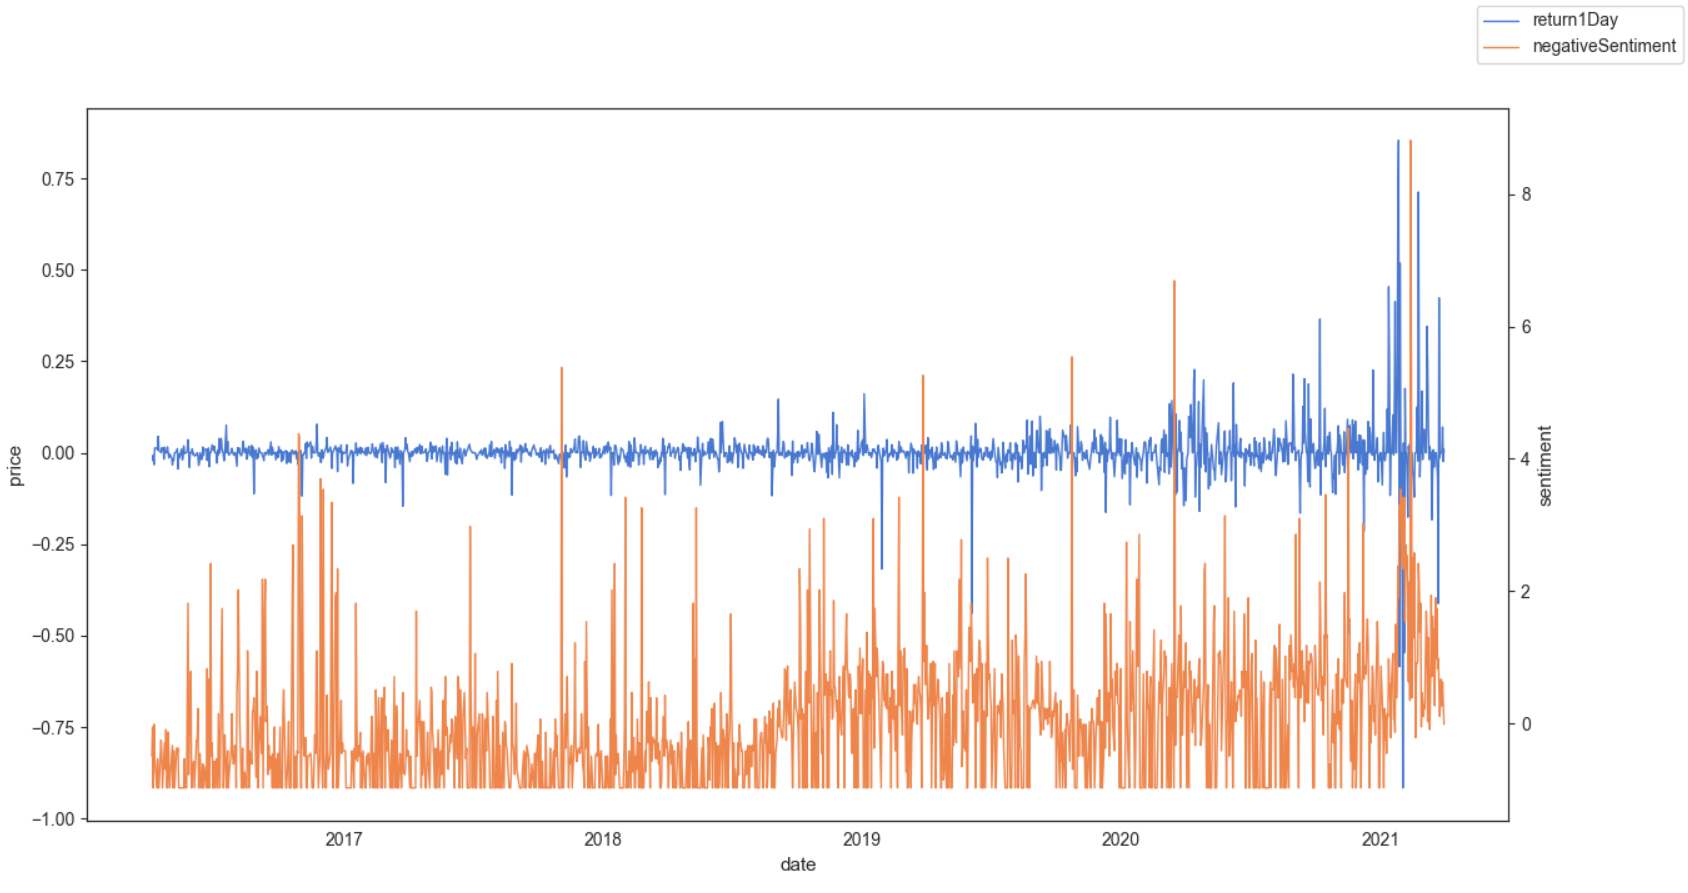
\includegraphics[width=15cm,height=7cm,keepaspectratio]{resultsEvaluation/1returnVsNeg.png}
    \caption{1 Day Returns Vs Negative Sentiment with entire data-set}
    \label{fig:1returnVsNeg}
\end{figure}

This graph shows that as the volatility of the returns increases, the negative sentiment increases. Indicating that there may be a potential relationship. It is also interesting to note that as of the end of 2018 the general negative sentiment level increased. It may be interesting to explore why this is the case.

\begin{center}
\begin{tabular}{ c|c|c }
\hline
\multicolumn{3}{|c|}{1 Day Return Vs Negative Sentiment Correlation with entire data-set} \\
\hline
Lag & \multicolumn{1}{|c|}{1 Day Return/Negative Sentiment} & \multicolumn{1}{|c }{Negative Sentiment/1 Day Return} \\
\hline
0 & & \\
1 & 0.0477 & \\
2 & & \\
3 & 0.0474 & \\
4 & & -0.0442 \\
5 & 0.0431 & -0.0444 \\
\end{tabular}
\end{center}

The first thing that is interesting to note is the relationship between the two directions of lag. It seems that 1 Day Return to Negative Sentiment has generally positive correlations, and for the opposing directions the opposite is true. This indicates the potential role of mean reversal, as if return increases negative sentiment will increase the next day, then the return will decrease in turn. It is also interesting to note that all of the values are very similar. The negative values even mirror the positive ones. This shows that the current return is related to what is said in the past few days as well as what will be said for a few days. It should also be noted that return positively correlates to negative sentiment and negative sentiment negatively correlates to returns. What these mean is that an increase in returns will correlate to an increase in negative sentiment, and an increase in negative sentiment correlates to a decreased level of returns.

\begin{figure}[h!]
    \centering
    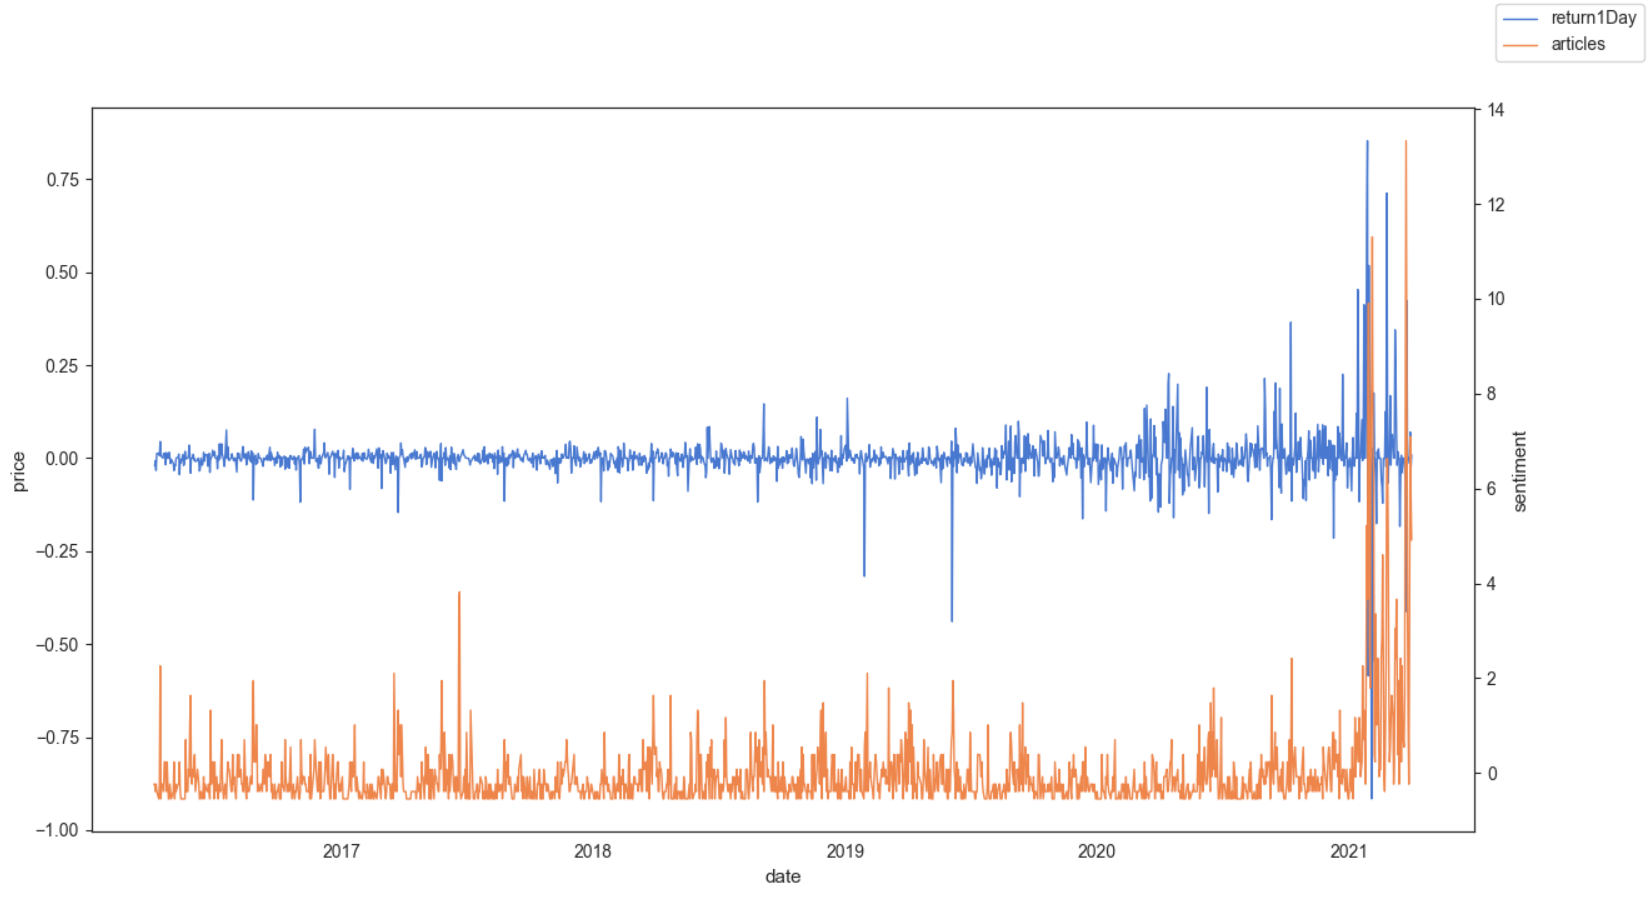
\includegraphics[width=15cm,height=7cm,keepaspectratio]{resultsEvaluation/1returnVsArticles.png}
    \caption{1 Day Returns Vs Article Volume with entire data-set}
    \label{fig:1returnVsArticle}
\end{figure}

This graph indicates that the large amount of return volatility recently works in tandem to a larger amount of articles that usual.

\begin{center}
\begin{tabular}{ c|c|c }
\hline
\multicolumn{3}{|c|}{1 Day Return Vs Article Volume Correlation with entire data-set} \\
\hline
Lag & \multicolumn{1}{|c|}{1 Day Return/Article Volume} & \multicolumn{1}{|c }{Article Volume/1 Day Return} \\
\hline
0 & & \\
1 & & \\
2 & 0.0926 & \\
3 & 0.0749 & \\
4 & & -0.07 \\
5 & 0.1267 & -0.0679 \\
\end{tabular}
\end{center}

It should be noted that returns positively correlates to article volume and article volume negatively correlates to returns. This indicates that if returns increase, article volume will too, however, if article volume increases returns will decrease. This is quite similar to the correlations between returns and negative sentiment.

\begin{center}
\begin{tabular}{ c|c|c }
\hline
\multicolumn{3}{|c|}{1 Day Return Vs Negative to Positive Sentiment Ratio Correlation with entire data-set} \\
\hline
Lag & \multicolumn{1}{|c|}{1 Day Return/Negative to Positive} & \multicolumn{1}{|c }{Negative to Positive/1 Day Return} \\
\hline
0 & & \\
1 & & \\
2 & -0.0476 & \\
3 & 0.0721 & \\
4 & -0.0615 & \\
5 & & \\
\end{tabular}
\end{center}

The positive to negative sentiment ratio correlation to 1 day returns was explored. This gave a few insights. It seems that this ratio does not correlate to future returns in a statistically significant way. However, the reverse is not true. The interesting part is that for the three days with statistically significant results the direction of influence is inconsistent, while maintaining a similar absolute value.

\section{Vector Auto-regression}

Finally all of this will be put together to explore causation. The full data-sets are stored in appendix \ref{appendix:vectorAutoregression}. The first three vector auto-regression use only one more variable on top of 1 day returns. The variables are then added on starting with the one which will have the greatest effect. This enable all of the variable explored to be added, and allows to see how much of an effect these have.

\begin{center}
\begin{tabular}{ c|c c|c|c c c }
\hline
\multicolumn{7}{|c|}{VAR Comparisons} \\
\hline
& \multicolumn{2}{|c|}{Lag Selection} & Unit root Test & \multicolumn{3}{|c }{VAR} \\
\hline
Name & AIC & Lag & asymptotic p-value & f-value & p-value & augmented $R^2$ \\
\hline
1 Day Return & 0.113197 & 6 & 5.185e-043 & 13.75066 & 1.68e-27 & 0.086788\\
Positive Sentiment & 0.113197 & 6 & 5.969e-026 & 11.78705 & 3.92e-23 & 0.074417 \\
\hline
1 Day Return & -0.014553 & 9 & 3.842e-034 & 10.82126 & 8.07e-27 & 0.089024 \\
Negative Sentiment & -0.014553 & 9 & 9.545e-014 & 24.22991 & 2.17e-64 & 0.187747 \\
\hline
1 Day Return & -0.719845 & 9 & 2.87e-033 & 11.11346 & 1.33e-30 & 0.101754 \\
Article Volume & -0.719845 & 9 & 8.907e-009 & 130.6266 & 3.0e-297 & 0.592161 \\
\hline
1 Day Return & 1.863201 & 9 & 2.87e-033 & 7.870976 & 1.64e-28 & 0.103495 \\
Article Volume & 1.863201 & 9 & 8.907e-009 & 16.08440 & 2.60e-65 & 0.202196 \\
Negative Sentiment & 1.863201 & 9 & 9.545e-014 & 88.52368 & 1.5e-292 & 0.595228 \\
\hline
1 Day Return & 4.279104 & 10 & 2.049e-028 & 5.850417 & 7.63e-27 & 0.107786 \\
Article Volume & 4.279104 & 10 & 8.052e-007 & 11.44909 & 3.48e-62 & 0.206507 \\
Negative Sentiment & 4.279104 & 10 & 1.107e-009 & 60.29136 & 7.8e-284 & 0.596244 \\
Positive Sentiment & 4.279104 & 10 & 5.969e-026 & 4.332794 & 2.42e-17 & 0.076646
\end{tabular}
\end{center}

From the examined models, the best fitting model is Negative Sentiment estimation from 1 Day Return, Article Volume, Negative Sentiment and Positive Sentiment, with an Adjusted $R^2$ of 0.596244. Meanwhile the most accurate model which estimates 1 Day Returns has an Adjusted $R^2$ of 0.107786 and is estimated from 1 Day Return, Article Volume, Negative Sentiment and Positive Sentiment.

\section{Machine Learning Exploration}

The various machine learning models are run against each other. The models are compared in figure \ref{fig:modelCompare}.

\begin{figure}[h!]
    \centering
    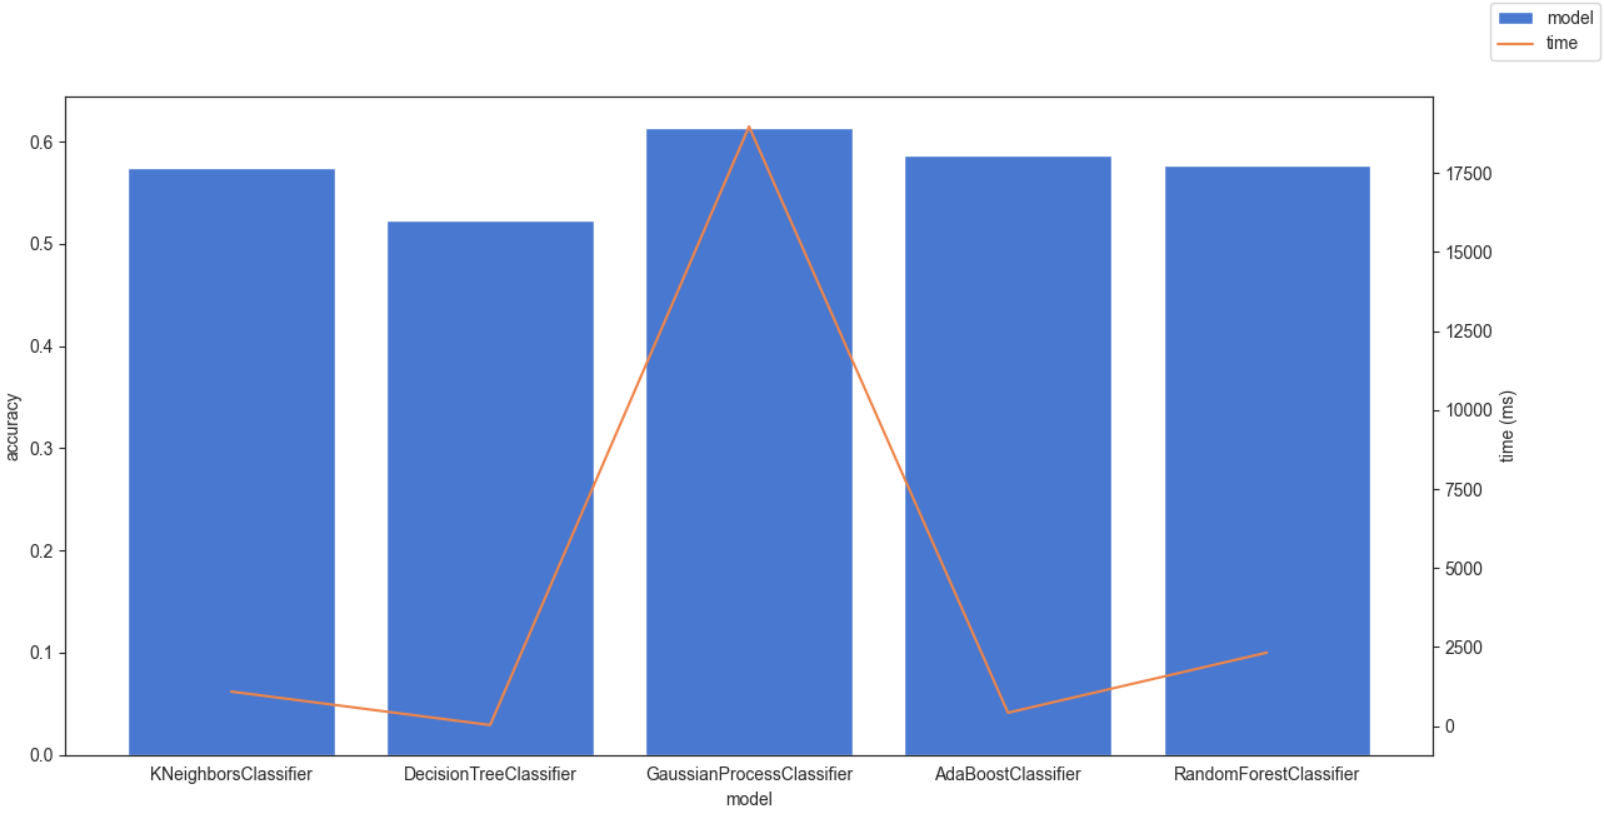
\includegraphics[width=15cm,height=7cm,keepaspectratio]{resultsEvaluation/modelCompare.png}
    \caption{Model Comparison}
    \label{fig:modelCompare}
\end{figure}

The model selector returns the GaussianProcessClassifier, with a 61.34\% accuracy. However, looking at figure \ref{fig:modelCompare}, it may have been wise to select the AdaBoostClassifier due to it's similar accuracy, 58.71\%, but significant training speed advantage that is 18974 ms against 420 ms training times.

%TODO direct comparison?

\section{Results Evaluation Summary}

This chapter uses the results provided by the system to explore the questions posed for this project.